\documentclass[11pt]{article}
\usepackage[margin=1in]{geometry}
\usepackage{amsmath,amssymb,booktabs,graphicx,float,hyperref,microtype,xcolor}
\usepackage[numbers]{natbib}
\usepackage{siunitx}
\usepackage{enumitem}
\hypersetup{colorlinks=true,linkcolor=blue,citecolor=blue,urlcolor=blue}
\graphicspath{{../figures/}}
\title{Geometry-Dependent Equilibria in Generalized Lennard--Jones-Type Power-Law Systems\\\large A Reproducible Theoretical and Computational Study}
\author{Toni Mladenovski\\Independent Researcher}
\date{11 November 2026\\Version 0.1.2 (publication candidate; not final)}

\begin{document}
\maketitle

\begin{abstract}
We study how a generalized inverse-power repulsive/stabilizing force law changes when pairwise interactions are projected through finite symmetric geometries. For
\[
F(r)=\frac{A}{r^n}-\frac{B}{r^m},\qquad A,B>0,\ n>m>0,
\]
the two-body equilibrium is $R_{\mathrm{EQ}}=(A/B)^{1/(n-m)}$. We define a radial geometry factor $G_{\mathcal G}(p)$ and obtain the geometry-dependent equilibrium
\[
R_{\mathrm{EQ}}^{(\mathcal G)}=\left[\frac{A\,G_{\mathcal G}(n)}{B\,G_{\mathcal G}(m)}\right]^{1/(n-m)}.
\]
Using the reference choice $A/B=2$, $n=13$, and $m=7$, we perform two reproducible computational experiments. Experiment 1 scans regular polygons from $N=3$ through $1000$ and compares five Platonic solids. Regular simplex geometries exhibit exact cancellation of the geometry ratio, while non-simplex geometries produce modest shifts. Within the computed $N=3,\ldots,1000$ scan, the polygon sequence has a unique minimum at $N=4$ for the reference exponent pair (no global theorem for all $N\ge3$ is claimed), and it approaches the analytic large-$N$ limit
\[
R_\infty=\left[2\,\frac{\zeta(12)}{\zeta(6)}\right]^{1/6}=1.1192958791\ldots.
\]
Under nearest-neighbor rescaling this is a local infinite-chain limit with curvature-weighted radial projections, not a conventional unit-projection chain sum and not a finite-radius continuum-circle force integral. Experiment 2 deforms a cube to a cuboid $(1,1,\delta)$. The two previously compared distance normalizations are shown to be exactly related by a change of length unit, while the deformed cuboid generally has a nonzero tangential force residual; its reported $R$ is therefore a constrained radial equilibrium, not a full vector equilibrium. We also prove a geometry bound for co-spherical configurations under nearest-neighbor normalization. A separately proposed interval $0.9\le R\le1.3$ is audited but not derived; it remains a heuristic operational window. The work is presented as a mathematical/computational model, not as experimental validation of new physics.
\end{abstract}

\section{Introduction}
Inverse-power interaction laws are historically central to molecular modeling. The early work of J. E. Jones introduced repulsive and attractive inverse-power descriptions of intermolecular fields \citep{Jones1924I,Jones1924II}; the now-standard Lennard--Jones (LJ) 12--6 form remains a canonical pair potential and has been extensively studied in molecular simulation, cluster optimization, and condensed-matter modeling \citep{SchwerdtfegerWales2024,WalesDoye1997,Romero1999}. Computational studies of such potentials also form part of the broader history of numerical statistical mechanics \citep{Metropolis1953}.

The present work does not seek a new fit to experimental intermolecular data. Instead, it asks a narrower mathematical question: if a generalized inverse-power force is radially projected through a finite geometry, how does the equilibrium radius depend on that geometry? This question separates into three components: (i) an analytic force-balance relation, (ii) a geometry-dependent projection factor, and (iii) a reproducible numerical exploration of selected geometry families.

A secondary motivation is methodological. During exploratory modeling, it is easy to mistake a numerically close value for a derived constant. We therefore maintain a strict provenance separation between quantities that are analytically derived, parameters chosen for a reference model, and externally proposed heuristic thresholds. In particular, the interval $[0.9,1.3]$ is treated as a working hypothesis only; no match is accepted as a derivation unless the criterion is independently motivated before numerical comparison.

\section{Generalized Force Model}
Consider
\begin{equation}
F(r)=\frac{A}{r^n}-\frac{B}{r^m},
\end{equation}
with $A,B>0$ and $n>m>0$. The equilibrium condition $F(R_{\mathrm{EQ}})=0$ gives
\begin{equation}
R_{\mathrm{EQ}}=\left(\frac{A}{B}\right)^{1/(n-m)}.
\end{equation}
For the reference ratio $A/B=2$ with $n=13$ and $m=7$,
\begin{equation}
R_{\mathrm{EQ}}=2^{1/6}=1.1224620483\ldots.
\end{equation}
This exponent pair corresponds structurally to the force obtained by differentiating a normalized LJ 12--6 potential,
\begin{equation}
V(R)=4(R^{-12}-R^{-6}).
\end{equation}
The use of $n=13,m=7$ in this paper is therefore a reference choice, not an empirical determination for the proposed geometry model.

\begin{figure}[H]
\centering
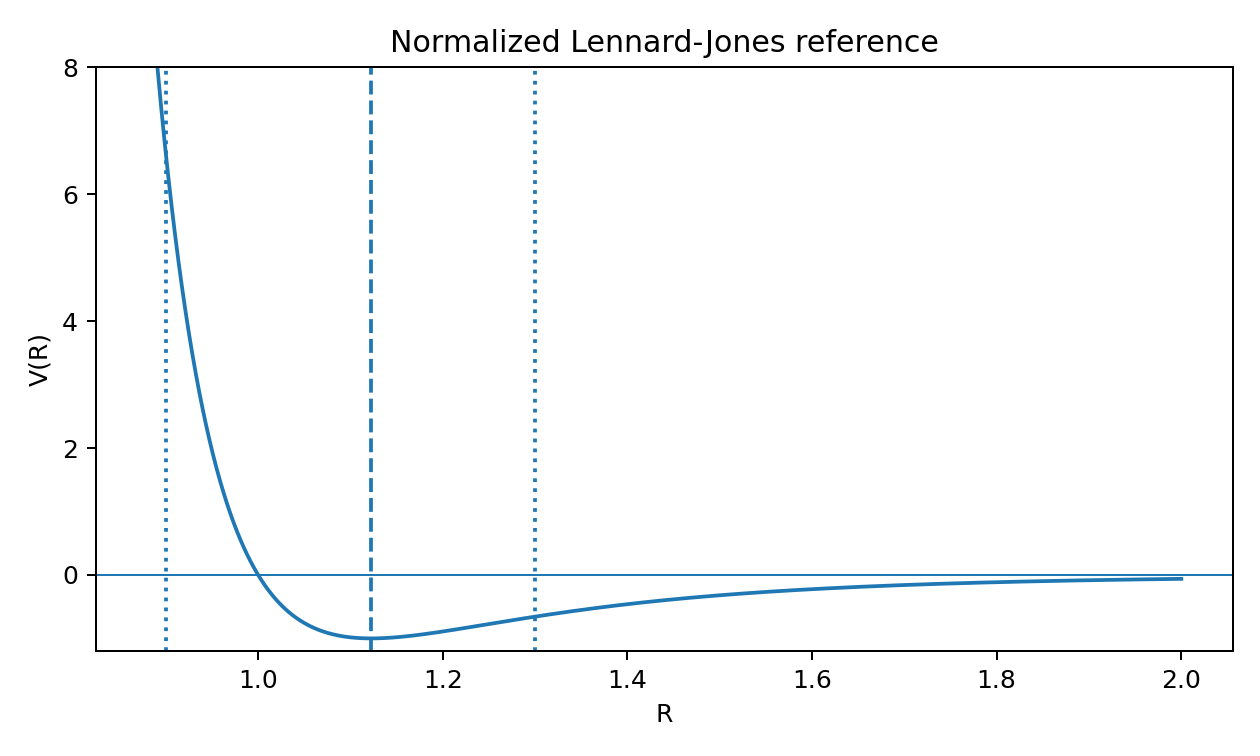
\includegraphics[width=0.78\textwidth]{figure_01_lj_reference.png}
\caption{Normalized LJ reference potential, the derived pair equilibrium, and the externally specified heuristic interval.}
\end{figure}

\section{Radial Geometry Factor}
Let $\mathcal G=\{\mathbf x_1,\dots,\mathbf x_N\}$ be a finite point configuration with centroid $\mathbf c$. Choose a source vertex $\mathbf x_i$. For each $j\ne i$, let $d_{ij}=\|\mathbf x_j-\mathbf x_i\|$, define a reference distance $d_{\mathrm{ref}}$, and set $\rho_{ij}=d_{ij}/d_{\mathrm{ref}}$. Let $\theta_{ij}$ be the angle between the direction toward $\mathbf x_j$ and the inward radial direction from $\mathbf x_i$ to $\mathbf c$. We define
\begin{equation}
G_{\mathcal G}(p)=\sum_{j\ne i}\frac{\cos\theta_{ij}}{\rho_{ij}^{p}}.
\end{equation}
For vertex-transitive geometries and a symmetric normalization, the result does not depend on the chosen vertex. The projected radial force is modeled as
\begin{equation}
F_{\mathcal G}(r)=G_{\mathcal G}(n)\frac{A}{r^n}-G_{\mathcal G}(m)\frac{B}{r^m},
\end{equation}
so that
\begin{equation}
\boxed{R_{\mathrm{EQ}}^{(\mathcal G)}=\left[\frac{A\,G_{\mathcal G}(n)}{B\,G_{\mathcal G}(m)}\right]^{1/(n-m)}}.
\end{equation}
It is convenient to define
\begin{equation}
Q_{\mathcal G}=\frac{G_{\mathcal G}(n)}{G_{\mathcal G}(m)},
\qquad
R_{\mathrm{EQ}}^{(\mathcal G)}=\left[(A/B)Q_{\mathcal G}\right]^{1/(n-m)}.
\end{equation}
Thus the geometry dependence is completely encoded by $Q_{\mathcal G}$ within this model.

\subsection{Simplex cancellation}
If every other vertex lies at the same normalized distance from the source, the factor $\rho_{ij}^{-p}$ is common to all terms. For the nearest-neighbor normalization of a regular simplex, $\rho_{ij}=1$ for every pair from the source. Hence $G_{\mathcal G}(p)$ is independent of $p$ and
\begin{equation}
Q_{\mathcal G}=1.
\end{equation}
Therefore the reference equilibrium is preserved exactly. This applies to the equilateral triangle in two dimensions and the regular tetrahedron in three dimensions under the declared construction.

\section{Experiment 1: Geometry Spectrum}
\subsection{Methods}
We evaluated $G_{\mathcal G}(13)$ and $G_{\mathcal G}(7)$ numerically using Cartesian vertex coordinates and direct radial projection. Distances were normalized by the nearest-neighbor distance. The experiment comprised:
\begin{enumerate}[nosep]
\item regular polygons for $N=3,\dots,1000$;
\item the tetrahedron, cube, octahedron, icosahedron, and dodecahedron.
\end{enumerate}
The geometry list and scan range are explicitly recorded in the release scripts. This package does not claim documentary proof that those choices were historically fixed before all exploratory comparisons.

\subsection{Regular polygons}
For a regular $N$-gon, the chord distances from a reference vertex can be expressed through $\sin(\pi k/N)$. With nearest-neighbor normalization,
\begin{equation}
\rho_k=\frac{\sin(\pi k/N)}{\sin(\pi/N)},
\end{equation}
and the inward radial projection is $\sin(\pi k/N)$. Hence
\begin{equation}
G_N(p)=\sin^p\left(\frac{\pi}{N}\right)\sum_{k=1}^{N-1}\sin^{1-p}\left(\frac{\pi k}{N}\right).
\end{equation}
The reference equilibrium is
\begin{equation}
R_{\mathrm{EQ}}(N)=\left[2\frac{G_N(13)}{G_N(7)}\right]^{1/6}.
\end{equation}

Within the computed scan $N=3,\ldots,1000$, the sequence has a unique minimum at $N=4$,
\begin{equation}
R_{\mathrm{EQ}}(4)=1.1126198392,
\end{equation}
after which the sampled sequence rises monotonically through $N=1000$. This is a finite-scan result, not a proof of a global minimum over all $N\ge3$. At $N=1000$,
\begin{equation}
R_{\mathrm{EQ}}(1000)=1.1192957642,
\end{equation}
which agrees with the analytic large-$N$ limit derived below. The $3$--$6$--$9$ subset is not exceptional in the complete sequence; it lies on the ordinary post-minimum branch.

\begin{figure}[H]
\centering
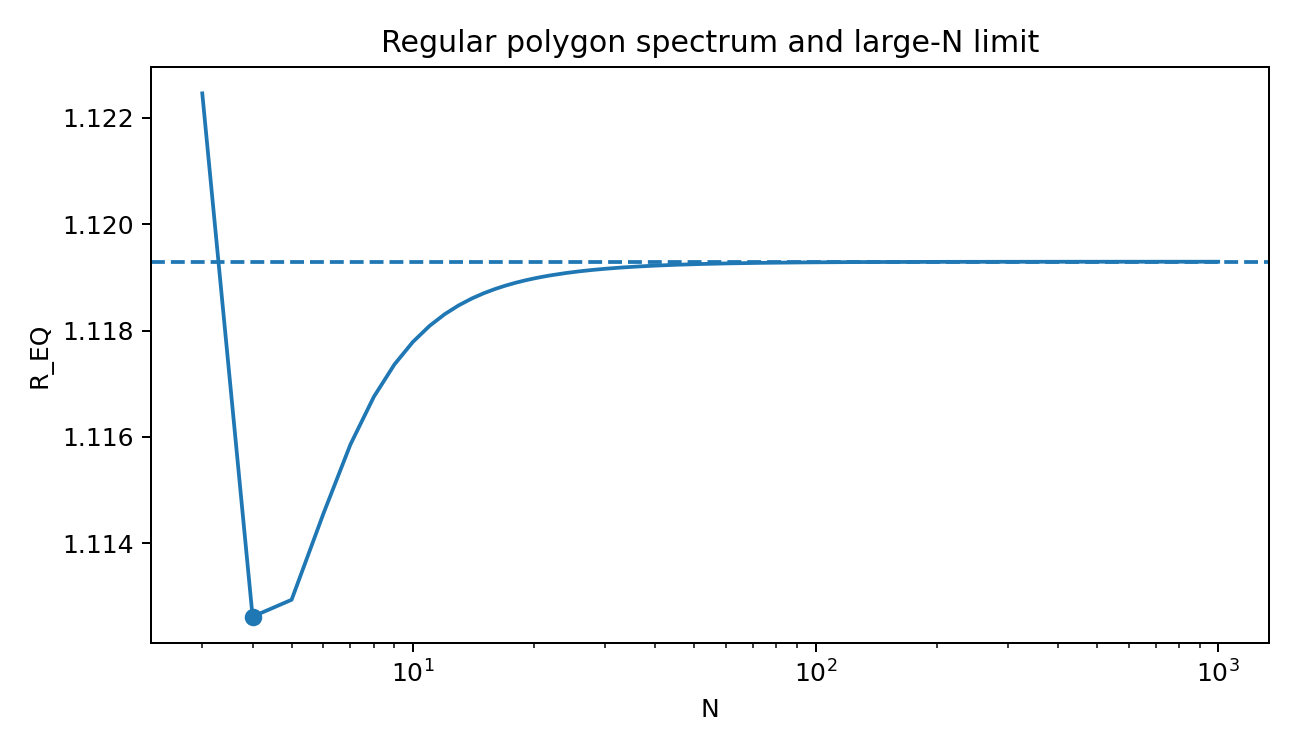
\includegraphics[width=0.82\textwidth]{figure_02_polygon_spectrum.png}
\caption{Regular-polygon scan for the reference exponent pair $(13,7)$. The unique minimum within the computed $N=3,\ldots,1000$ scan occurs at $N=4$, followed by smooth convergence toward the analytic large-$N$ limit. The logarithmic horizontal axis displays both the low-$N$ structure and large-$N$ convergence.}
\end{figure}


\subsection{Analytic large-$N$ limit}
Throughout this subsection assume $n>m>2$. For fixed integer $k$ as $N\to\infty$,
\[
\sin(\pi/N)\sim \frac{\pi}{N},\qquad
\sin(\pi k/N)\sim \frac{\pi k}{N}.
\]
Each end of the polygon sum contributes terms asymptotic to $(\pi/N)k^{1-p}$. For $p>2$ the fixed-$k$ sums converge, and the two ends give
\begin{equation}
G_N(p)\sim \frac{2\pi}{N}\,\zeta(p-1)\qquad(p>2).
\end{equation}
Therefore, for $n>m>2$,
\begin{equation}
\boxed{R_\infty=\left[(A/B)\frac{\zeta(n-1)}{\zeta(m-1)}\right]^{1/(n-m)}},\qquad n>m>2.
\end{equation}
The condition $p>2$ is essential: $\zeta(p-1)$ diverges at $p=2$, and the endpoint-dominated asymptotic changes for $p\le2$. The regimes $m<2$ and $m=2$ are not derived here, and the accompanying \texttt{polygon\_limit()} function rejects $m\le2$.
For $(A/B,n,m)=(2,13,7)$,
\begin{equation}
R_\infty=\left[2\frac{\zeta(12)}{\zeta(6)}\right]^{1/6}=1.1192958791\ldots.
\end{equation}
Because nearest-neighbor normalization shrinks the physical reference length as $N$ grows, the rescaled local environment approaches an infinite one-dimensional chain. Thus the limiting formula is best interpreted as a local infinite-chain limit induced by nearest-neighbor rescaling, not as the force integral of a fixed-radius continuous circle. The interpretation requires one qualification: for fixed $k$ the inward radial projection $\sin(\pi k/N)\sim\pi k/N$ vanishes, so $G_N(p)=O(1/N)$ and the coefficient $\zeta(p-1)$ is curvature-weighted. It is therefore not the conventional infinite-chain sum with unit radial projection, which would give $2\zeta(p)$.

\subsection{A bound for co-spherical configurations}
Suppose all vertices lie on one sphere centered at the centroid, nearest-neighbor normalization is used, all radial projection weights are nonnegative, and $n>m>0$. Then $1\le\rho_j\le\rho_{\max}$ and
\[
\rho_{\max}^{-(n-m)}\rho_j^{-m}\le \rho_j^{-n}\le \rho_j^{-m}.
\]
Multiplying by the nonnegative projection weights and summing yields
\[
\rho_{\max}^{-(n-m)}\le \frac{G(n)}{G(m)}\le1.
\]
Consequently,
\begin{equation}
\boxed{\frac{R_{\rm ref}}{\rho_{\max}}\le R_{\rm EQ}^{(\mathcal G)}\le R_{\rm ref}},
\end{equation}
where $R_{\rm ref}=(A/B)^{1/(n-m)}$. In particular, for the reference model, $R_{\rm EQ}^{(\mathcal G)}\le2^{1/6}<1.3$ throughout this admissible class. Thus the upper heuristic boundary $1.3$ is rigorously unreachable by this geometry mechanism under the stated assumptions.

\subsection{Platonic solids}
Table~\ref{tab:platonic} summarizes the five tested regular solids.
\begin{table}[H]
\centering
\caption{Geometry factors and equilibrium radii for tested Platonic solids.}
\label{tab:platonic}
\begin{tabular}{lrrrr}
\toprule
Geometry & $G(13)$ & $G(7)$ & $Q$ & $R_{\mathrm{EQ}}$\\
\midrule
Tetrahedron & 2.449490 & 2.449490 & 1.000000 & 1.122462\\
Cube & 1.759906 & 1.969941 & 0.893380 & 1.101567\\
Octahedron & 2.839476 & 2.916815 & 0.973485 & 1.117446\\
Icosahedron & 2.637054 & 2.786246 & 0.946454 & 1.112214\\
Dodecahedron & 1.077231 & 1.208751 & 0.891193 & 1.101117\\
\bottomrule
\end{tabular}
\end{table}

\begin{figure}[H]
\centering
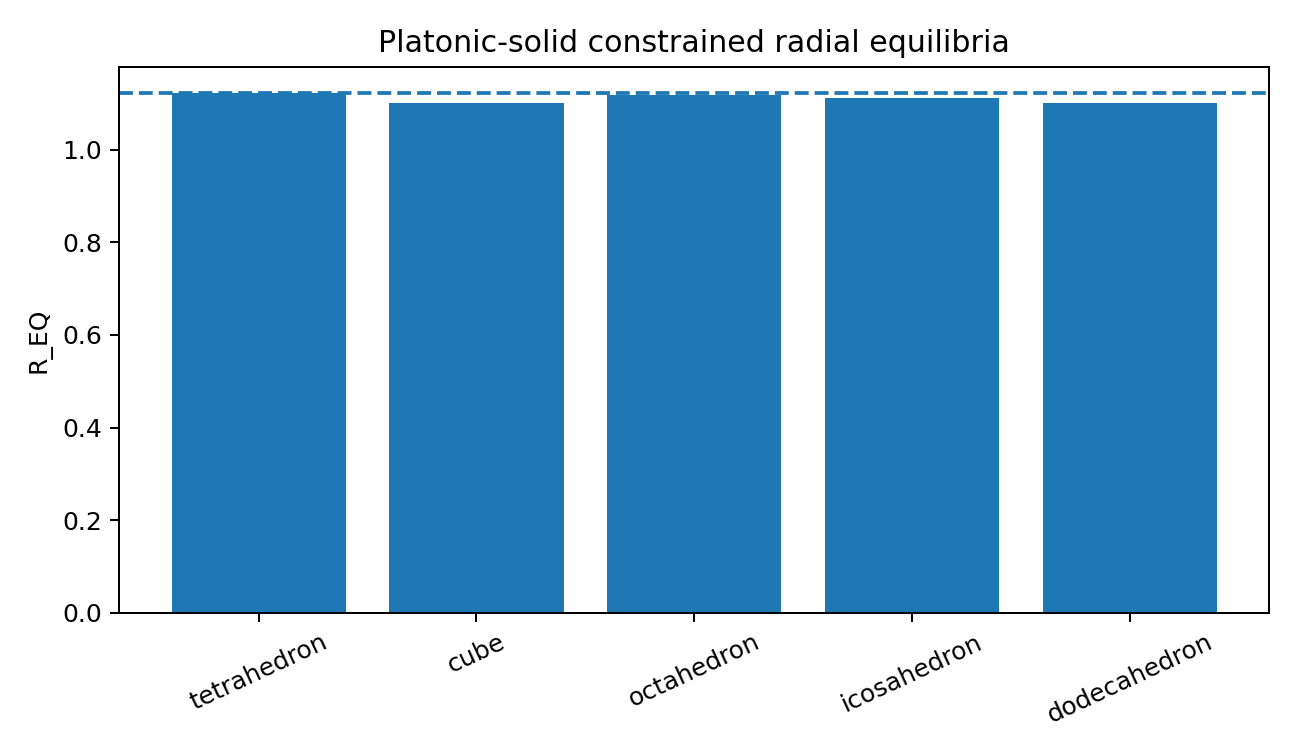
\includegraphics[width=0.8\textwidth]{figure_03_platonic_spectrum.png}
\caption{Reference equilibrium radii for the five tested Platonic solids.}
\end{figure}

These results show a genuine but modest geometry-induced equilibrium shift. In the tested regular families, the effect is insufficient to span the much broader heuristic interval $[0.9,1.3]$.

\section{Experiment 2: Controlled Cuboid Deformation}
\subsection{Motivation and interpretation}
We deform the cube to a cuboid with half-axis lengths $(1,1,\delta)$, $\delta>0$. The radial geometry equation still produces a scalar value $R_{\rm EQ}^{(\mathcal G)}$, but for $\delta\ne1$ the full vector-force sum is generally not radial. The quantity reported here is therefore a \emph{constrained radial equilibrium}: the inward radial projection vanishes while a tangential residual may remain.

Two reference-length conventions were retained in the code for audit purposes: nearest-neighbor distance $d_{\rm nn}$ and a fixed reference $d_{\rm fixed}=2$. They are not independent physical models. Because $G(p)$ scales as $d_{\rm ref}^{p}$, the corresponding equilibrium coordinates satisfy exactly
\begin{equation}
\boxed{R_{\rm fixed}=R_{\rm near}\frac{d_{\rm fixed}}{d_{\rm nn}}}.
\end{equation}
The release verifies this identity numerically over all 601 sampled cuboids to machine precision. A value near $1.3$ in fixed-edge units is therefore a coordinate rescaling of the same configuration, not a separate prediction or boundary derivation.

\subsection{Results}
With nearest-neighbor units over the 409-point deformation scan, the constrained radial equilibrium reaches a minimum near
\begin{equation}
\delta\approx0.85134,\qquad R_{\rm radial}\approx1.04725.
\end{equation}
At this same shape, direct summation of the full vector pair forces gives zero radial component to numerical precision but a nonzero tangential residual. With the common normalized-LJ force prefactor $24$, the residual magnitude is approximately $9.24$ in the corresponding force units. Thus the deformed cuboid is not in unconstrained vector equilibrium at this radial root.

\begin{figure}[H]
\centering
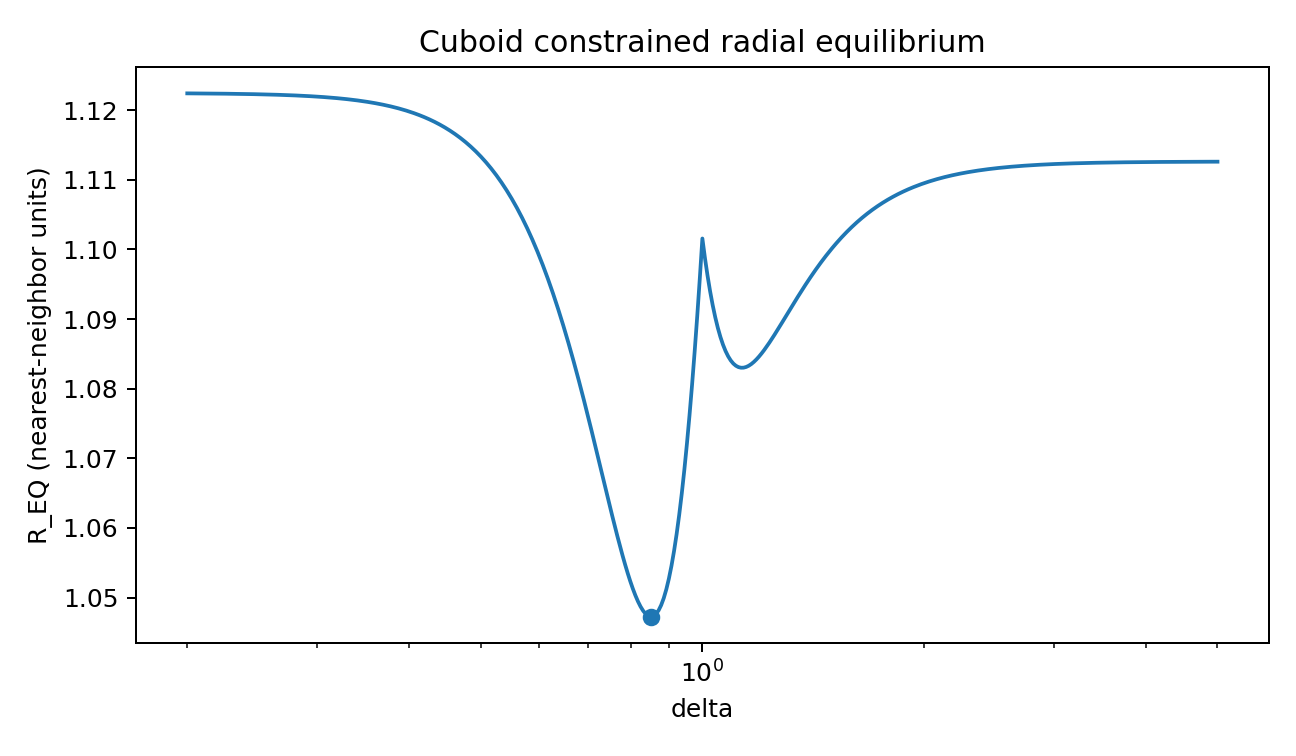
\includegraphics[width=0.82\textwidth]{figure_04_cuboid_deformation.png}
\caption{Constrained radial equilibrium for the cuboid deformation in nearest-neighbor length units. For $\delta\ne1$, the radial root need not be a full vector equilibrium.}
\end{figure}

\begin{figure}[H]
\centering
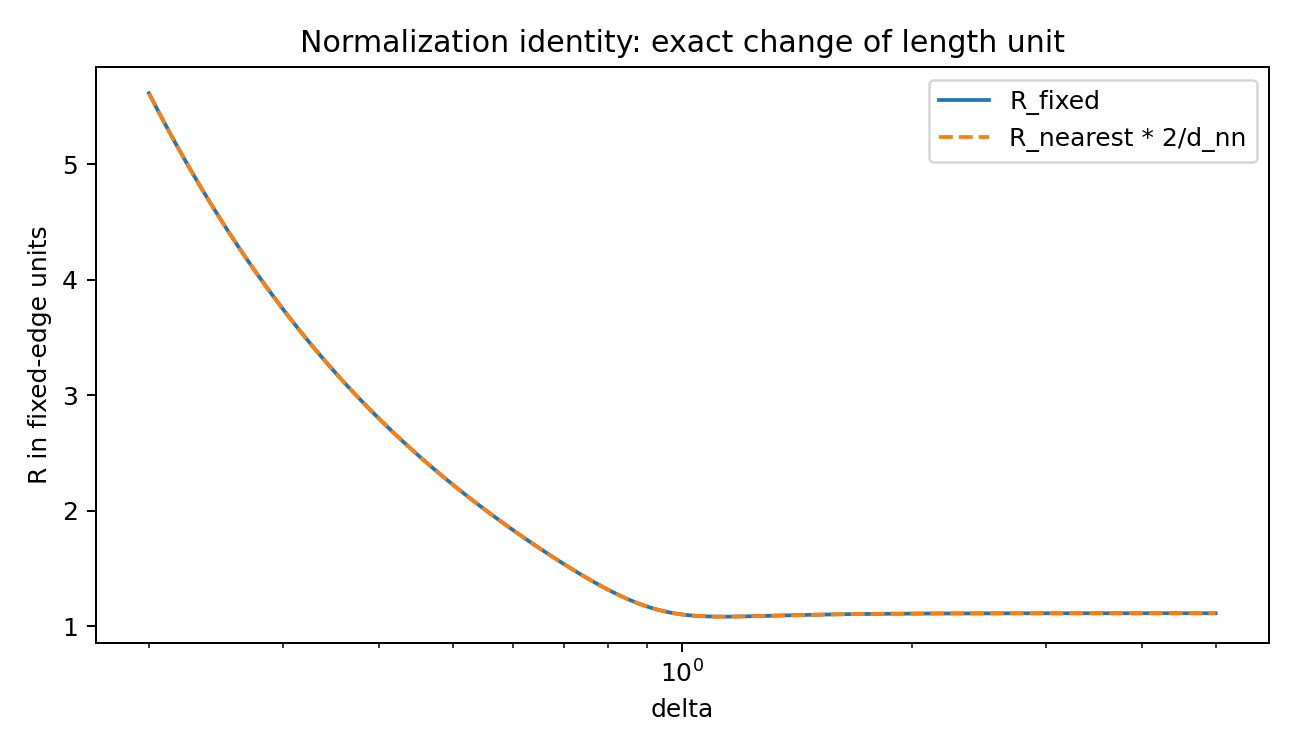
\includegraphics[width=0.82\textwidth]{figure_06_normalization_sensitivity.png}
\caption{Exact normalization identity. The fixed-edge coordinate coincides with $R_{\rm near}(2/d_{\rm nn})$ to machine precision, demonstrating a change of length unit rather than two independent physical predictions.}
\end{figure}

The main inference from Experiment 2 is therefore twofold: controlled deformation can substantially alter the constrained radial root, but the root alone does not establish full mechanical equilibrium; and apparent differences caused solely by $d_{\rm ref}$ conventions must be interpreted as unit rescalings.

\section{Boundary Audit}
A separate exploratory framework proposed the operational interval
\begin{equation}
0.9\le R\le1.3.
\end{equation}
The present study treats these numbers as hypotheses, not outputs. Several independent checks were used during model development, including the LJ zero at $R=1$, the curvature transition
\begin{equation}
R=\left(\frac{26}{7}\right)^{1/6}\approx1.24446,
\end{equation}
and geometry-driven shifts. None provides a single independently motivated criterion that derives both endpoints. Regular geometry spectra remain near $1.10$--$1.12$. Controlled deformation can move the constrained radial root farther, but a fixed-edge value near $1.3$ is exactly a rescaling of the nearest-neighbor coordinate. Moreover, the co-spherical bound proves that $1.3$ cannot be reached by the nearest-neighbor-normalized geometry mechanism under its stated assumptions.

We therefore record the provenance as follows:
\begin{itemize}[nosep]
\item $R_{\mathrm{EQ}}=2^{1/6}$: analytically derived for the reference two-body model;
\item $R_{\mathrm{EQ}}^{(\mathcal G)}$: derived from the declared geometry-factor model;
\item $0.9$ and $1.3$: heuristic operational thresholds, not derived constants.
\end{itemize}

\section{Discussion}
The geometry-factor formulation produces several useful structural insights. First, equal-distance simplices cancel the exponent dependence of the geometry factor, preserving the reference equilibrium. Second, non-simplex geometries with multiple distance shells generally produce $G(n)\ne G(m)$ and therefore shift equilibrium. Third, adding vertices alone does not guarantee a larger shift: the complete regular-polygon scan occupies a very narrow interval and converges smoothly. Fourth, controlled deformation is more effective than increasing polygon order for the constrained radial root, but generally leaves a tangential force residual when the shape is not radially symmetric.

The normalization audit also changes the interpretation of the deformation study. A change of $d_{\rm ref}$ rescales the reported equilibrium coordinate exactly; it does not generate a new dimensionless physical state. Comparisons across deformations therefore require one declared unit convention. In this paper the nearest-neighbor convention is used for the primary geometry comparisons, while fixed-edge values are retained only to demonstrate the exact rescaling identity.

The results also clarify what this study does not establish. It does not show that actual atoms, gravitational systems, or information channels obey the geometry factor introduced here. It does not experimentally validate an EIT/H-space model. It does not derive the heuristic thresholds. The contribution is a reproducible mathematical architecture and a set of positive and negative computational results that can be independently audited.

\section{Limitations and Open Problems}
Key open questions include:
\begin{enumerate}
\item How do polygon extrema change for general exponent pairs $(n,m)$? The $N=4$ minimum is a result for the reference $(13,7)$ pair, not a universal theorem.
\item What sharper bounds can be proved for restricted geometry classes beyond the co-spherical nearest-neighbor bound established here?
\item Which deformed geometries admit a simultaneous zero of the full vector force, rather than only the radial projection?
\item How should the model be reformulated if the shape itself is allowed to relax dynamically rather than being externally fixed?
\item Can extrema of the full vector-equilibrium problem be characterized analytically for non-simplex families?
\end{enumerate}

\paragraph{Scope note.} The earlier exploratory label ``P2-SMOOTH $a=b=2$'' belongs to a separate energy-partition sandbox and is not part of the geometry-equilibrium model studied or implemented in this release. Version 0.1.1 states this explicitly to prevent cross-module provenance confusion.

\section{Reproducibility and Research Integrity}
The accompanying research package contains source code, two experiment scripts, regression tests, generated CSV/JSON data, figures, a checksum manifest, citation metadata, and independent-review prompts. Version 0.1.1 adds \texttt{scripts/build\_all.py}, which deterministically regenerates all committed data products and figures from the declared source model. Build caches, compiled Python files, LaTeX auxiliary files, and duplicate PDFs are excluded from the release archive. (The v0.1.1 archive inadvertently still contained cache and bytecode files; they are removed in v0.1.2.)

AI-assisted tooling was used in the iterative development of code, exposition, and consistency checks. No external AI system is listed as an independent reviewer unless an actual review report is obtained and archived. Prepared prompts for Claude, Kimi, Tasklet, or other systems are included as an adversarial-review protocol. An author-supplied Kimi independent AI review of v0.1.1 (verdict: pass with corrections) is archived in \texttt{review/}; its five required corrections are addressed in v0.1.2. These AI reviews are not scientific peer review. A Tasklet review summary supplied by the author for v0.1.0 is archived separately and is explicitly labeled as AI review rather than scientific peer review. Human authorship remains responsible for the claims and for deciding what is published.

\section{Conclusion}
A generalized inverse-power force can be extended to a geometry-dependent constrained radial equilibrium through a projected factor $G_{\mathcal G}(p)$. Within the reference $(13,7)$ model, regular simplices preserve the original equilibrium exactly, while non-simplex geometries shift it. Within the computed $N=3,\ldots,1000$ scan, regular polygons have a unique minimum at $N=4$ for this exponent pair (not a global theorem), and they approach the analytic large-$N$ local-chain limit (curvature-weighted projections) $[2\zeta(12)/\zeta(6)]^{1/6}=1.1192958791\ldots$. For co-spherical configurations with nearest-neighbor normalization, the bound $R_{\rm ref}/\rho_{\max}\le R_{\rm EQ}^{(\mathcal G)}\le R_{\rm ref}$ proves that, for the reference parameters, the upper heuristic threshold $1.3$ cannot arise within this nearest-neighbor-normalized co-spherical class; it does not exclude $1.3$ for other normalizations, non-co-spherical geometries, or other model choices. Controlled cuboid deformation can move the radial root farther, but generally leaves a tangential force residual; alternate reference-length normalizations are exactly related by unit rescaling. Consequently, $0.9$ and $1.3$ remain heuristic rather than derived. The main result is a reproducible framework with explicit limits on what the geometry model does and does not establish.

\begin{figure}[H]
\centering
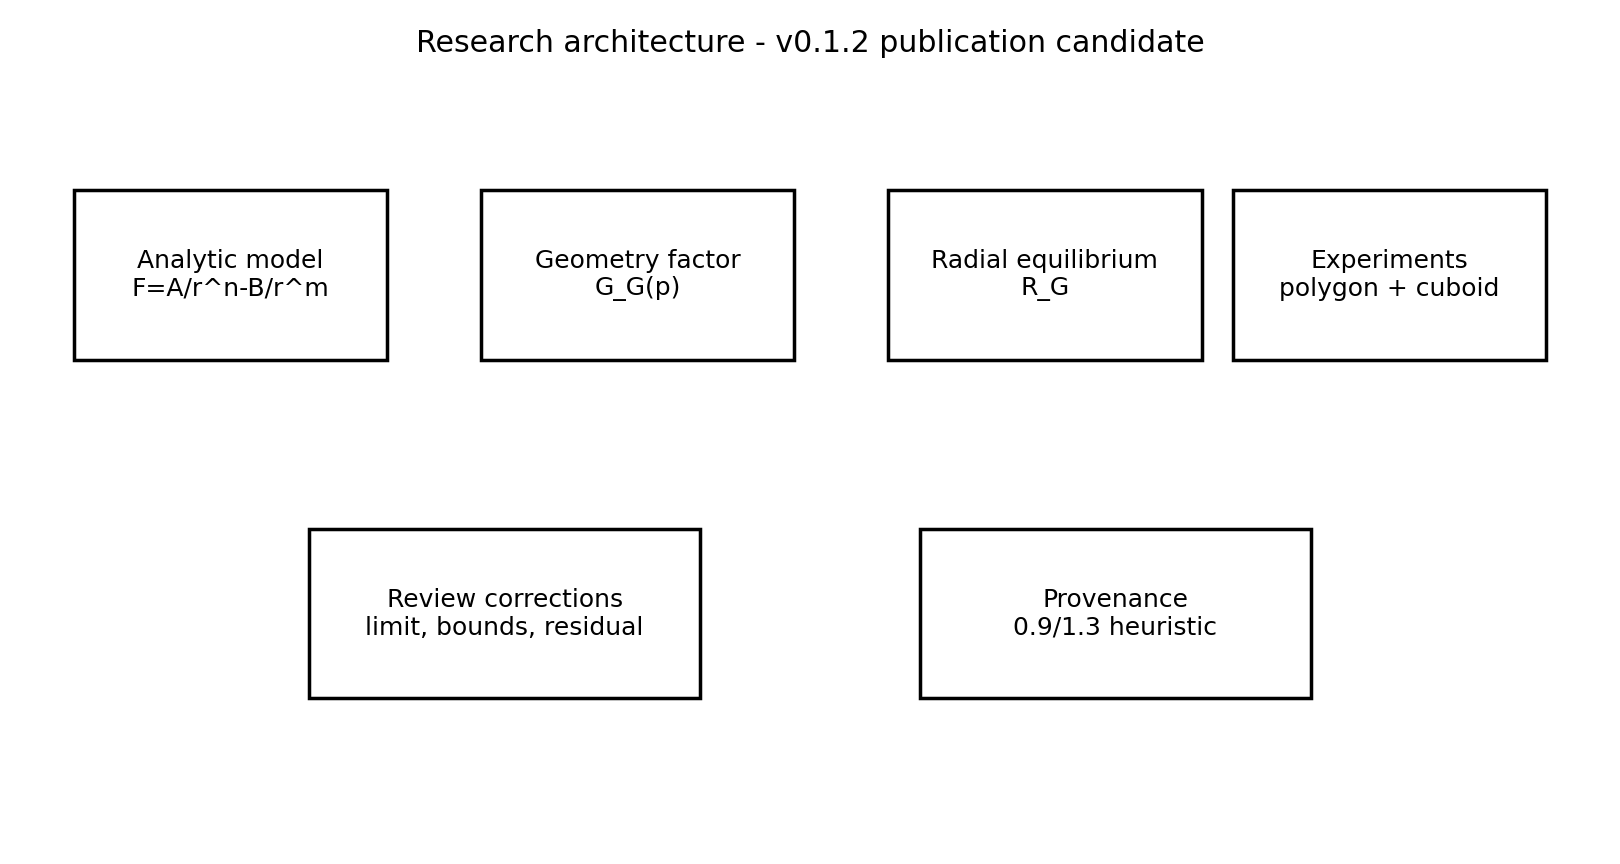
\includegraphics[width=0.9\textwidth]{figure_05_research_architecture.png}
\caption{Research architecture emphasizing separation of analytic derivation, computational geometry, boundary audit, and provenance.}
\end{figure}

\paragraph{Licensing.} Code in this release is distributed under PolyForm Noncommercial 1.0.0; the manuscript, figures, and documentation are distributed under CC BY-NC-SA 4.0.
% Canonical bibliography source (rendered). paper/references.bib is a convenience BibTeX export kept in sync.
\begin{thebibliography}{9}
\bibitem{Jones1924I} J. E. Jones, ``On the Determination of Molecular Fields. I. From the Variation of the Viscosity of a Gas with Temperature,'' \emph{Proc. R. Soc. Lond. A}, 106(738), 441--462 (1924). DOI: 10.1098/rspa.1924.0081.
\bibitem{Jones1924II} J. E. Jones, ``On the Determination of Molecular Fields. II. From the Equation of State of a Gas,'' \emph{Proc. R. Soc. Lond. A}, 106(738), 463--477 (1924). DOI: 10.1098/rspa.1924.0082.
\bibitem{SchwerdtfegerWales2024} P. Schwerdtfeger and D. J. Wales, ``100 Years of the Lennard-Jones Potential,'' \emph{J. Chem. Theory Comput.}, 20(9), 3379--3405 (2024). DOI: 10.1021/acs.jctc.4c00135.
\bibitem{WalesDoye1997} D. J. Wales and J. P. K. Doye, ``Global Optimization by Basin-Hopping and the Lowest Energy Structures of Lennard-Jones Clusters Containing up to 110 Atoms,'' \emph{J. Phys. Chem. A}, 101(28), 5111--5116 (1997). DOI: 10.1021/jp970984n.
\bibitem{Romero1999} D. Romero, C. Barron, and S. Gomez, ``The Optimal Geometry of Lennard-Jones Clusters: 148--309,'' \emph{Comput. Phys. Commun.}, 123, 87--96 (1999). DOI: 10.1016/S0010-4655(99)00259-3.
\bibitem{Metropolis1953} N. Metropolis, A. W. Rosenbluth, M. N. Rosenbluth, A. H. Teller, and E. Teller, ``Equation of State Calculations by Fast Computing Machines,'' \emph{J. Chem. Phys.}, 21(6), 1087--1092 (1953). DOI: 10.1063/1.1699114.
\end{thebibliography}
\end{document}
